\chapter{Visualização Estereoscópica}

O InVesalius suporta visualização estereoscópica de modelos 3D, para isso é necessário criar uma superfície (ver capítulo~\ref{cap_surface}) ou uma visualização volumétrica ativa (ver capítulo~\ref{cap:vis_vol}), em seguida ir clicar no ícone que a figura~\ref{fig:ster} mostra, no lado direito parte inferior do InVesalius e escolher o tipo de projeção desejada (figura~\ref{fig:st_menu}). 

\begin{figure}[!htb]
\centering

\includegraphics[scale=0.6]{3D_glasses.png}
\caption{Atalho para ativar os métodos de visualização estereoscópica.}
\label{fig:ster}
\end{figure}

\begin{figure}[!htb]
\centering
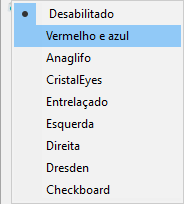
\includegraphics[scale=0.4]{st_menu.png}
\caption{Diferentes métodos de visualização estereoscópica.}
\label{fig:st_menu}
\end{figure}

O InVesalius suporta os seguintes tipos de visualização estereoscópica:

\begin{itemize}
	\item Vermelho e azul
	\item Anaglifo
	\item \textit{CristalEyes}
	\item Entrelaçado
	\item Esquerda
	\item Direita
	\item Dresden
	\item Checkboard
\end{itemize}

A figura~\ref{fig:st_surf_methods} apresenta três diferentes tipos de projeções.

\begin{figure}[!htb]
  \centering
  \subfloat[Entrelaçado]{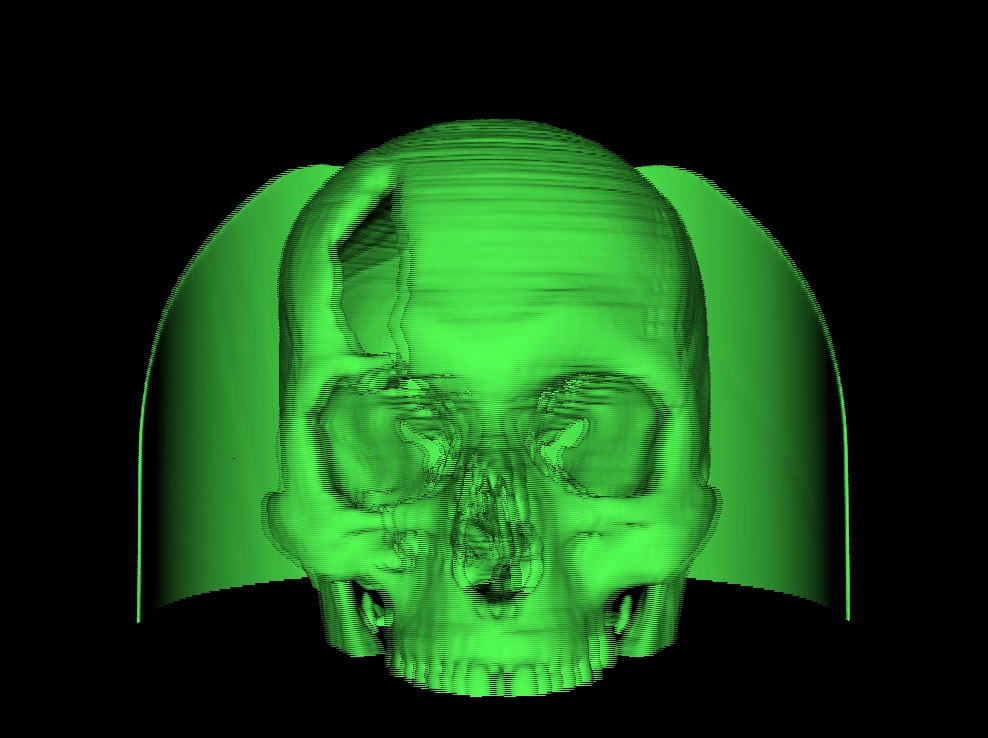
\includegraphics[width=0.3\textwidth]{st_surf_interlaced.jpg}} \qquad
  \subfloat[Anaglifo]{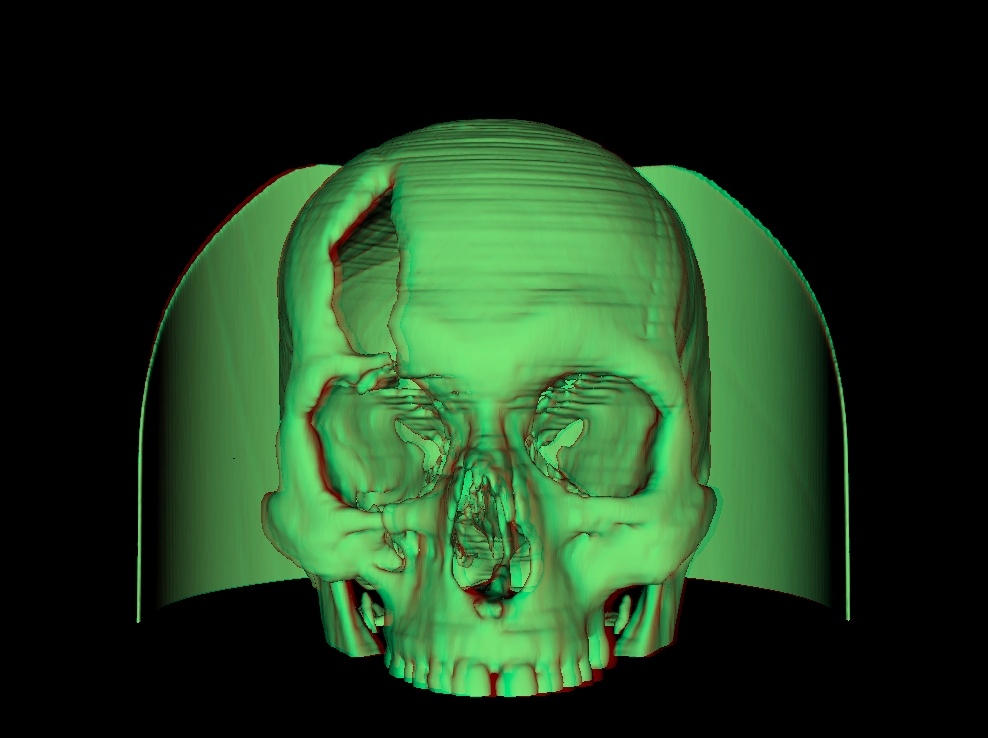
\includegraphics[width=0.3\textwidth]{st_surf_anaglyph.jpg}} \qquad
  \subfloat[Vermelho e azul]{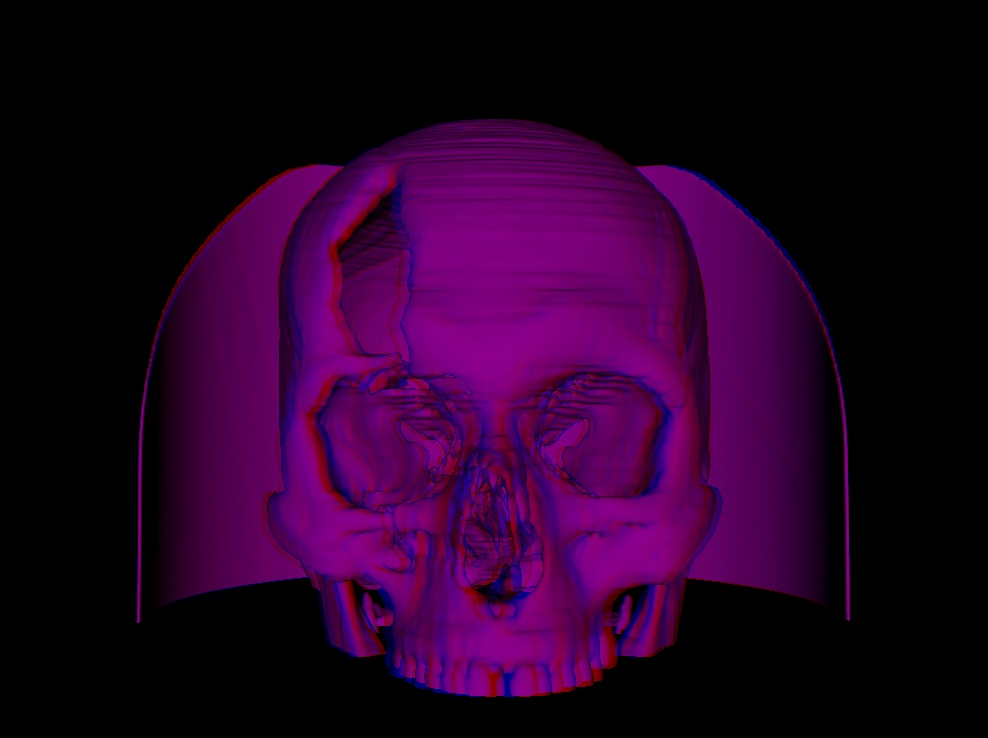
\includegraphics[width=0.3\textwidth]{st_surf_red_blue.jpg}}  
  \hfill
  \caption{Exemplo de diferentes métodos de estereoscópica aplicado em uma superfície.}
  \label{fig:st_surf_methods}
\end{figure}